Informacje na obrazie są wyświetlane za pomocą obiektów \sokarclass{SceneIndicator}.
Obiekty te mają dostęp do bazy danych obrazu DICOM i odpowiednio zmieniają swoją zawartość.

Domyślnie obiekty wyświetlające informacje:
\begin{itemize}

    \item \sokarclass{PatientDataIndicator}

    Obiekt wyświetlający dane pacjenta, pojawia się od zawsze na obrazie w lewym górnym rogu i zawiera następujące linie:
    \begin{itemize}
        \item Nazwa pacjenta oraz płeć

        Nazwa pacjenta znajduje się w \dicomtag{PatientName}{0010}{0010} o \dicomvr{PN}.
        
        Płeć, zapisana jest w \dicomtag{PatientSex}{0010}{0040} i może mieć następujące wartości:
        \begin{itemize}
            \item \quotett{M } - oznacza mężczyznę, wyświetlana jako O
            \item \quotett{F } - oznacza kobietę, wyświetlana jako O
            \item \quotett{O } - oznacza inną płeć i nie jest wyświetlana
        \end{itemize}
        
        W przypadku określenia inne płci niż jest w standardzie bądź braku tagu płeć nie będzie widoczna.

        Przykład: \quotett{Adam Jędrzejowski O}.

        \item Identyfikator pacjenta

        Unikalny identyfikator pacjenta z tagu \dicomtag{PatientID}{0010}{0020} wyświetlane w takiej formie jakiej jest zapisane, bez żadnej obróbki.
        W praktyce najczęściej jest to numer z systemu używanego w danym szpitalu, rzadziej numer pesel.
        
        Przykład: \quotett{HIS/000000}.

        \item Data urodzenia oraz wiek pacjenta w trakcie badania

        Data urodzenia znajdująca się w \dicomtag{PatientBirthDate}{0010}{0030} i jest zamieniana na format \quotett{YYYY-MM-DD}.
        Dodatkowo, jeżeli tag \dicomtag{PatientAge}{0010}{1010} jest obecny wyświetlany jest także wiek pacjenta w czasie badania.
    
        Przykład: \quotett{born 1982-08-09, 28 years}.

        \item Opis wykonany przez instytucję opis lub klasyfikację badania (komponentu)
        
        Tekst brany z \dicomtag{StudyDescription}{0008}{1030} i wyświetlany bez żadnej obróbki.

        UWAGA: Ta wartość jest wpisywana przez technika, operatora lub lekarza wykonującego badanie, więc wartość ta może być nie przewidywalna.

        \item Opis serii
        
        Tekst brany z \dicomtag{SeriesDescription}{0008}{103E} i wyświetlany bez żadnej obróbki.
        
        UWAGA: Ta wartość jest wpisywana przez technika, operatora lub lekarza wykonującego badanie, więc wartość ta może być nie przewidywalna.
    \end{itemize}

    Przykład pełnego teksu:
    
    \texttt{\textbf{Adam Jędrzejowski} O\\
    HIS/123456\\
    born 1996-07-16, 19 years\\
    Kregoslup ledzwiowy a-p + boczne\\
    AP
    }
    
    \item \sokarclass{HospitalDataIndicator}
    
    Obiekt wyświetlający dane szpitala/instytucji, pojawia się od zawsze na obrazie w prawym górnym rogu i zawiera następujące linie:
    \begin{itemize}
        \item Nazwa instytucji
        
        Tekst brany z \dicomtag{InstitutionalDepartmentName}{0008}{1040} i wyświetlany bez żadnej obróbki.
        
    \end{itemize}

    \item \sokarclass{ImageOrientationIndicator}

    Obiekt wyświetlający cztery litery oznaczające orientacje obrazu w stosunku do pacjenta, przykład można zobaczyć na rysunku \ref{fig:imageorientationindicator1}.
    Obiekt posiada cztery pola: lewe, górne, prawe i dolne.

    \begin{figure}[h]
        \caption{
            Przykład jak wygląda \sokarclass{ImageOrientationIndicator} w praktyce.
            Widzimy tu, że lewa strona pacjenta znajduje się po prawej stronie obrazu, prawa strona pacjenta po lewej, góra pacjenta na górnej części obrazu.
            Wynika z tego, że obraz przedstawia pacjenta skierowanego twarzą do nas.
            }
        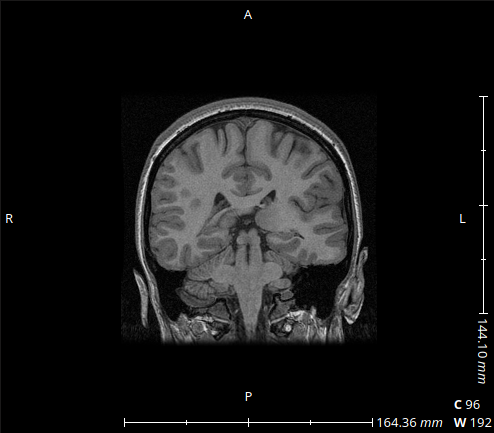
\includegraphics[width=\textwidth]{img/imageorientationindicator-002.png}
        \centering
        \label{fig:imageorientationindicator1}
    \end{figure}
    
    Każda z sześciu możliwych liter oznacza kierunek oraz zwrot w jakim jest ułożony pacjent:
    \begin{itemize}
        \item \quotett{R} - right - część prawa pacjenta
        \item \quotett{L} - left - część 
        \item \quotett{A} - anterior - przód pacjenta
        \item \quotett{P} - posterior - tył pacjenta
        \item \quotett{F} - feet - część dolna
        \item \quotett{H} - head - część górna
    \end{itemize}

    Pary poszczególnych liter tworzą osie:
    \begin{itemize}
        \item \quotett{x} - oś przechodząca od prawej do lewej strony pacjenta, \quotett{L} oznacza zwrot zgodny z osią, a \quotett{R} oznacza zwrot przeciwny, wizualizacja na rysunku \ref{fig:imageorientationindicator2}

        \begin{figure}[h]
            \caption{Wizualizacja osi \quotett{x} pacjenta}
            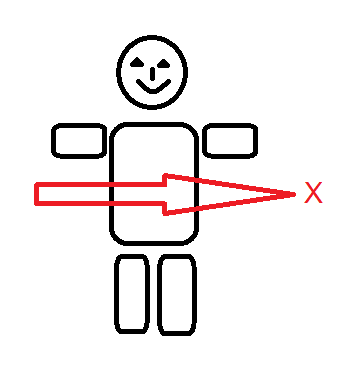
\includegraphics[]{img/imageorientationindicator-101.png}
            \centering
            \label{fig:imageorientationindicator2}
        \end{figure}

        \item \quotett{y} - oś przechodząca od przodu do tył pacjenta, \quotett{P} oznacza zwrot zgodny z osią, a \quotett{A} oznacza zwrot przeciwny, wizualizacja na rysunku \ref{fig:imageorientationindicator3}

        \begin{figure}[h]
            \caption{Wizualizacja osi \quotett{y} pacjenta}
            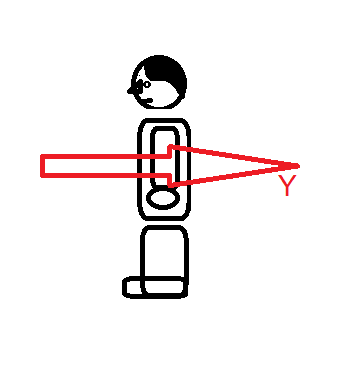
\includegraphics[]{img/imageorientationindicator-102.png}
            \centering
            \label{fig:imageorientationindicator3}
        \end{figure}

        \item \quotett{z} -  - oś przechodząca od dołu do góry pacjenta, \quotett{H} oznacza zwrot zgodny z osią, a \quotett{F} oznacza zwrot przeciwny, wizualizacja na rysunku \ref{fig:imageorientationindicator4}

        \begin{figure}[h]
            \caption{Wizualizacja osi \quotett{z} pacjenta}
            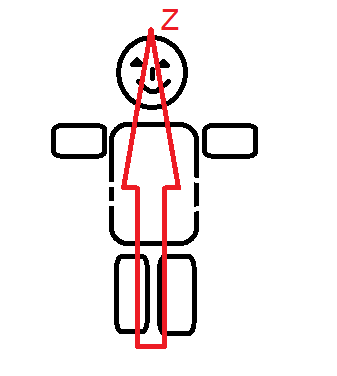
\includegraphics[]{img/imageorientationindicator-103.png}
            \centering
            \label{fig:imageorientationindicator4}
        \end{figure}

    \end{itemize}

    Informacje o orientacji oraz pozycji względem pacjenta znajdują się w odpowiednio w tagach \dicomtag{ImageOrientation}{0020}{0037} i \dicomtag{ImagePosition}{0020}{0032}.
    Wartość \dicomtag{ImageOrientation}{0020}{0037} składa się z sześciu liczb, opowiednio oznaczanych dalej X\textsubscript{x}, X\textsubscript{y}, X\textsubscript{z}, Y\textsubscript{x}, Y\textsubscript{y}, Y\textsubscript{z}.

    Standard DICOM definiuje, że te dane mają być z interpretowane w następujący sposób:    
    \[
        \begin{bmatrix}
            P_x \\ P_y \\ P_z \\ 1
        \end{bmatrix}
        =
        \begin{bmatrix}
            X_x\Delta_i & Y_x\Delta_j & 0 & S_x \\
            X_y\Delta_i & Y_y\Delta_j & 0 & S_y \\
            X_z\Delta_i & Y_z\Delta_j & 0 & S_z \\
            0 & 0 & 0 & 1
        \end{bmatrix}
        \begin{bmatrix}
            i \\ j \\ 0 \\ 1
        \end{bmatrix}
        =
        M
        \begin{bmatrix}
            i \\ j \\ 0 \\ 1
        \end{bmatrix}
    \]
    gdzie:
    \begin{conditions}
    P_{xyz} & The coordinates of the voxel (i,j) in the frame's image plane in units of mm.\\
    S_{xyz} & The three values of Image Position (Patient) (0020,0032). It is the location in mm from the origin of the RCS.\\
    X_{xyz} & The values from the row (X) direction cosine of Image Orientation (Patient) (0020,0037).\\
    Y_{xyz} & The values from the column (Y) direction cosine of Image Orientation (Patient) (0020,0037).\\
    i & Column index to the image plane. The first column is index zero.\\
    \Delta_i & Column pixel resolution of Pixel Spacing (0028,0030) in units of mm.\\
    j & Row index to the image plane. The first row index is zero.\\    
    \Delta_j & Row pixel resolution of Pixel Spacing (0028,0030) in units of mm.
    \end{conditions}

    Brak tłumaczenia jest celowy, aby uniknąć nie porozumień.

    Wyjaśnienia:
    \begin{itemize}
        \item $P_{xyz}$ oznacza punkt pozycji pacjenta wyrażony w milimetrach
        \item $S_{xyz}$ oznacza punkt pozycji pacjenta wyrażony w milimetrach w stosunku do urządzenia wykonującego pomiar, dane brane z \dicomtag{ImagePosition}{0020}{0032}
        \item $X_{xyz}$ oznacza trzy pierwsze wartości z \dicomtag{ImageOrientation}{0020}{0037}
        \item $Y_{xyz}$ oznacza trzy ostatnie wartości z \dicomtag{ImageOrientation}{0020}{0037}
        \item $i$ i $j$ oznaczają współrzędne na obrazu
        \item $\Delta_i$ i $\Delta_j$ oznaczają rzeczywistą wielkość piksela obrazu wyrażoną w mm, w algorytmie wyznaczania strony pacjenta ta wartość, może wynosić 1, ponieważ odpowiada za skale
    \end{itemize}

    Praktycznie rzecz biorąc, pierwsza macierz to wektor reprezentujący pozycje pacjenta.
    Druga jest to transformata.
    Trzecia to pozycja na obrazie.
    
    Interesuje nas wyznaczenie pozycji sześciu (punktów) na płaszczyźnie obrazu, o następujących współrzędnych, dalej używanych pod nazwą $PatientPosition$:
    \begin{itemize}
        \item \quotett{R} - $[-1, 0, 0, 1]$
        \item \quotett{L} - $[+1, 0, 0, 1]$
        \item \quotett{A} - $[0, -1, 0, 1]$
        \item \quotett{P} - $[0, +1, 0, 1]$
        \item \quotett{F} - $[0, 0, -1, 1]$
        \item \quotett{H} - $[0, 0, +1, 1]$
    \end{itemize}

    UWAGA: Wszystkie obliczenia odbywają się w współrzędnych jednorodnych.

    Wykonuje takie przekształcenie:
    \[PatientPosition = imgMatrix * ScenePosition\]
	\[imgMatrix^{-1} * PatientPosition = imgMatrix^{-1} * imgMatrix * ScenePosition\]
	\[imgMatrix^{-1} * PatientPosition = ScenePosition\]
    \[ScenePosition = imgMatrix^{-1} * PatientPosition\]
    gdzie:
    \begin{conditions}
        imgMatrix & macierz przekształcenia obrazu, o której będzie dalej\\
        ScenePosition & pozycja na obrazie, która naz interesuje \\
        PatientPosition & któryś z punktów względem pacjenta.
    \end{conditions}

    Wygląd macierzy $imgMatrix$:
    \[
        \begin{bmatrix}
            X_x & Y_x & 0 & 0 \\
            X_y & Y_y & 0 & 0 \\
            X_z & Y_z & 0 & 0\\
            0 & 0 & 0 & 1
        \end{bmatrix}
    \]
    Powyższa macierz różni się od macierzy definiowanej w standardzie.
    Po pierwsze PikselSpacing został pominięty, a konkretniej nadałem mu wartość 1.
    Po drugie pozycja z \dicomtag{ImagePosition}{0020}{0032} została zrównana do punktu zerowego, dzięki temu, wynik też będzie względem punktu zero.
    Wyznaczenie macierzy $imgMatrix$ jest jednorazowe.

    Po wyznaczeniu sześciu punktów $ScenePosition$, po jednej dla każdego punktu względem pacjenta są zapisywane. $ScenePosition$ odpowiada pozycji punktów na obrazie w pozycji startowej.

    Na scenie, której jest wyświetlany obraz, użytkownik, może obracać obraz do woli, według własnego uznania.
    Te przekształcenia, są realizowane za pomocą macierzy rotacji, dalej znana jako $rotateTransform$.
    Macierz $rotateTransform$ jest przesyłana do naszego obiektu \sokarclass{ImageOrientationIndicator} za każdym razem kiedy zostanie zmieniona.

    Ostateczne wyznaczenie pozycji punktów pacjent na obrazie odbywa sie przez przemnożenie lewostronne $rotateTransform$ i $ScenePosition$.
    \[rotateTransform * ScenePosition\]
    Wyznaczane jest w ten sposób pozycja sześciu punktów pacjenta na płaszczyźnie sceny wyświetlanej.
    Następnie określane jest na, której z ośmiu części płaszczyzny jest umieszczony dany punkt, podział płaszczyzny jest widoczny na rysunku \ref{fig:imageorientationindicator5}.
    Tej płaszczyźnie nadawany jest tytuł w postaci litery, która oznacza punkt pacjenta.
    Jeżeli punkt znajduje się w centrum, na przecięciu osi, to oznacza, że punkt znajduje się za lub przed ekranem, więc jest pomijany.
    Następnie do czterech pól wyświetlających zostają wstawione następujące teksty:
    \begin{itemize}
        \item lewe pole: tytuł części 7, tytuł części 0 i tytuł części 1
        \item górne pole: tytuł części 1, tytuł części 2 i tytuł części 3
        \item prawe pole: tytuł części 3, tytuł części 4 i tytuł części 5
        \item dolne pole: tytuł części 7, tytuł części 6 i tytuł części 5
    \end{itemize}

    Przykład:\\
    Punkt \quotett{H}, czyli punkt reprezentujący kierunek głowy, został przypisany do części 1 i odpowiednio \quotett{L} do części 7, \quotett{R} do części 3 i \quotett{F} do części 5.
    Punkty \quotett{A} i \quotett{P} zostały pominięte ponieważ znalazły się na środku.
    Do lewego pola wstawiany jest tekst \quotett{HL}, do górnego \quotett{HR}, do prawego \quotett{RF} i do dolnego \quotett{LF}.

    \begin{figure}[h]
        \caption{Podział płaszczyzny sceny. Wyróżniono osiem części.}
        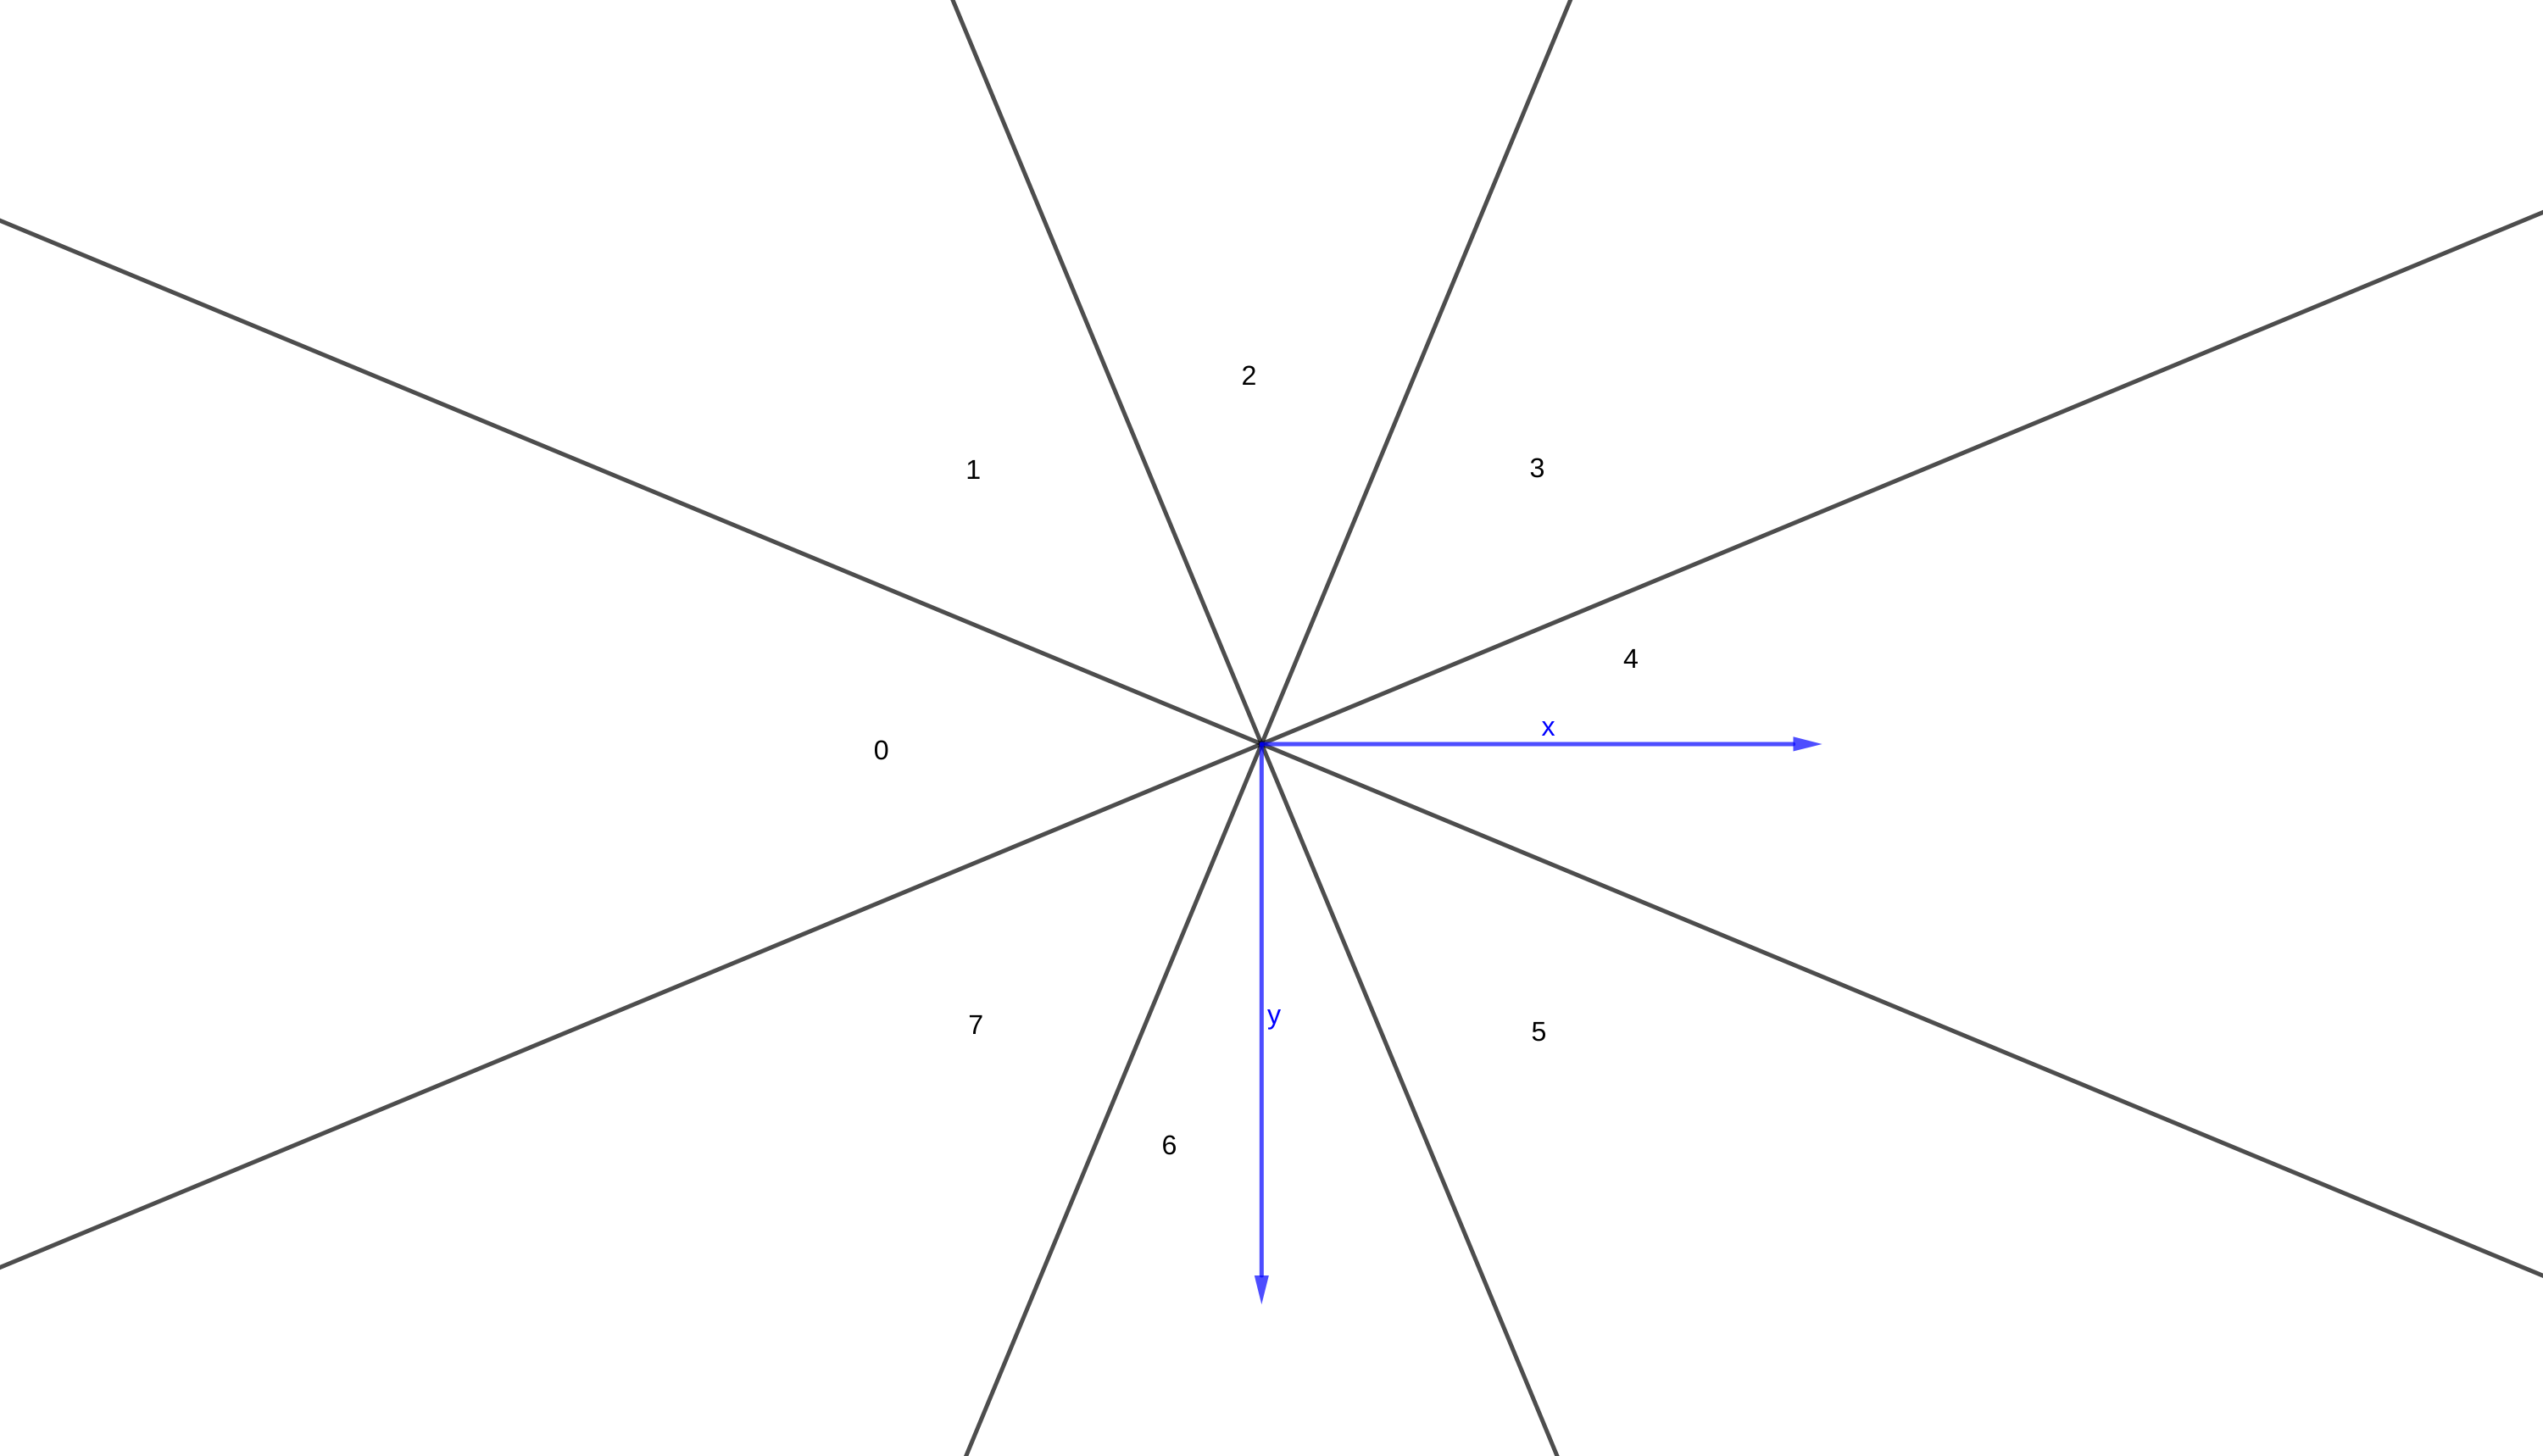
\includegraphics[width=\textwidth]{img/imageorientationindicator-300.png}
        \centering
        \label{fig:imageorientationindicator5}
    \end{figure}

    \item \sokarclass{PixelSpacingIndicator}
    
    Obiekt wyświetlający miarkę z podziałką informującą jakich rozmiarów jest obiekt na obrazie w rzeczywistości, pojawia się na dole i po prawie stronie sceny, gdy tag \dicomtag{PixelSpacing}{0028}{0030} jest obecny.
    Wygląd podziałki można zaobserwować na rysunku \ref{fig:imageorientationindicator1}.

    Podziałka dostosowuje swoją wielkość do obecnej sceny, jak i do innych elementów na scenie.
    Wartości wyświetlane biorą pod uwagę transformatę skali i rotacji obrazu.

    \item \sokarclass{ModalityIndicator}
    
    Obiekt wyświetla informacje o akwizycji obrazu.
    Dane różnią się w zależności od modalności obrazu.
    Domyślnie zawierają następujące linie:
    \begin{itemize}
        \item bla bla bla
        \item bla bla bla
        \item bla bla bla
        \item bla bla bla
    \end{itemize}

    W przypadku następujących modalności zawierają również następujące informacje:
    \begin{itemize}
        \item bla bla bla
        \item bla bla bla
        \item bla bla bla
        \item bla bla bla
    \end{itemize}
\end{itemize}
